\documentclass[10pt]{article}
\usepackage{newtxtext}
\usepackage{amsfonts,amsmath,amsthm,amssymb,mathtools}
\usepackage{bbm}
\usepackage{enumitem}
\usepackage{comment}
\usepackage{hyperref}
\usepackage{cleveref}
\usepackage[round]{natbib}
\usepackage[left=1in, right=1in, top=1in, bottom=1in]{geometry}
\usepackage{xcolor}
\usepackage{todonotes}
\usepackage{graphicx}
\usepackage{listings}
\usepackage{mathrsfs}
\usepackage{stmaryrd}
\usepackage[Symbol]{upgreek}
\usepackage{booktabs}
\usepackage[font=small]{caption}

% ==========================================
% COMMENTS TOGGLE
% ==========================================
\newif\ifshowcomments
% \showcommentstrue%  UNCOMMENT to show comments
\showcommentsfalse% UNCOMMENT to hide comments

% ==========================================
% METADATA
% ==========================================
\newcommand{\ProjectName}{Sheaf Enriched Autonomous Multi-Agent Networks (SEAMAN)}
\newcommand{\ProjectAbbrv}{SEAMAN}
\newcommand{\ReportName}{Milestone 4: Robot Demonstration}
\newcommand{\ProjectID}{HR0011-25-3-0235}
\newcommand{\Author}{Dr. Hans Riess (PI)}
\newcommand{\Date}{\today}

% HEADERS & FOOTERS
\usepackage{fancyhdr}
\setlength{\headheight}{20.37502pt}
\addtolength{\topmargin}{-8.37502pt}
\fancyhf{}
\fancyhead[L]{\footnotesize{\textit{\ReportName} \\ \ProjectID \\ \Date}}
\fancyfoot[C]{\footnotesize{\thepage}}
\renewcommand{\headrulewidth}{0pt} % Remove the header rule
\pagestyle{fancy}

% MATH
\renewcommand{\leq}{\leqslant}
\renewcommand{\geq}{\geqslant}
\renewcommand{\preceq}{\preccurlyeq}
\renewcommand{\succeq}{\succcurlyeq}
\newcommand{\face}{\trianglelefteqslant}
\newcommand{\coface}{\trianglerighteqslant}
\newcommand{\category}[1]{\mathsf{#1}}
\newcommand{\shf}{\mathscr{F}}
\newcommand{\Lap}{\mathcal{L}}
\newcommand{\coLap}{\mathcal{L}^{\scriptscriptstyle\vee}}
\newcommand{\Con}[1]{\text{Con}(#1)}
\newcommand{\sat}[1]{\overline{#1}}
\newcommand{\tile}{\mathsf{q}}
\graphicspath{{figures/}{../figures/}}

% COLORS
\definecolor{buzzgold}{HTML}{EAAA00}
\definecolor{riceblue}{HTML}{00205B}
\definecolor{rpired}{HTML}{D6001C}
\definecolor{techgold}{HTML}{B3A369}
\definecolor{navyblue}{HTML}{003057}
\definecolor{techgreen}{HTML}{22EE66}
\definecolor{techred}{HTML}{E04F39}

% PYTHON LISTINGS STYLE
\lstset{
  language=Python,
  basicstyle=\small\ttfamily,
  keywordstyle=\color{navyblue}\bfseries,
  commentstyle=\color{techgold!80!black},
  stringstyle=\color{techgreen!70!black},
  showstringspaces=false,
  breaklines=true,
  frame=lines,
  numbers=left,
  numberstyle=\tiny\color{gray},
  tabsize=4,
  captionpos=b,
}

%THEOREMS

\theoremstyle{definition}
\newtheorem{theorem}{Theorem}
\newtheorem{proposition}{Proposition}
\newtheorem{lemma}{Lemma}
\newtheorem{corollary}{Corollary}
\newtheorem{definition}{Definition}
\newtheorem{example}{Example}
\theoremstyle{remark}
\newtheorem{remark}{Remark}
\newtheorem{notation}{Notation}

% Command for tasks
\newcommand{\task}[1]{%
    \ifshowcomments
        ~\todo[inline, color=buzzgold!60, textcolor=black,caption={Task}]{{\bf Task:} #1}%
    \fi
}

% Official subtask language, always displayed (centered italics quote box)
\newcommand{\prompt}[1]{%
    \begin{quote}
        \centering\itshape #1
    \end{quote}%
}

\newcommand{\hans}[1]{%
    \ifshowcomments
        \noindent\textcolor{buzzgold}{[Hans]: #1}%
    \fi
}

\newcommand{\ai}[1]{%
    \ifshowcomments
        \noindent\textcolor{techred}{[AI Agent]: #1}%
    \fi
}


%%%%%%%%%%%%%%%%%%%%%%%%%%%%%%%%%%%%%%%%%%%%%%%%%%%%%%%%%%%%%%%%%%%%%%%%%%%%%%%%%%%
\title{{\huge\sffamily\bfseries \ProjectName} \\ \vspace{10pt} {\Large\it \ReportName} \\ \vspace{10pt} {\normalsize Submitted by~\Author}}
\date{}
%%%%%%%%%%%%%%%%%%%%%%%%%%%%%%%%%%%%%%%%%%%%%%%%%%%%%%%%%%%%%%%%%%%%%%%%%%%%%%%%%%%
%%%%%%%%%%%%%%%%%%%%%%%%%%%%%%%%%%%%%%%%%%%%%%%%%%%%%%%%%%%%%%%%%%%%%%%%%%%%%%%%%%%
\begin{document}
\maketitle
\tableofcontents
\vspace{1cm}
\thispagestyle{fancy}
%%%%%%%%%%%%%%%%%%%%%%%%%%%%%%%%%%%%%%%%%%%%%%%%%%%%%%%%%%%%%%%%%%%%%%%%%%%%%%%%%%%

%%%%%%%%%%%%%%%%%%%%%%%%%%%%%%%%%%%%%%%%%%%%%%%%%%%%%%%%%%%%%%%%%%%%%%%%%%%%%%%%%%%
\section{Introduction}
\label{sec:intro}
%%%%%%%%%%%%%%%%%%%%%%%%%%%%%%%%%%%%%%%%%%%%%%%%%%%%%%%%%%%%%%%%%%%%%%%%%%%%%%%%%%%

Autonomous multi-agent systems operating in contested environments must coordinate under intermittent, low-bandwidth communication while their constituent agents hold partial---and, more perniciously, mutually contradictory---beliefs about the world and about one another's objectives. The SEAMAN program addresses this challenge by modeling the information state of a multi-agent network as a \emph{cellular sheaf of assume-guarantee contracts} over the communication graph: each agent's knowledge and commitments constitute a local contract, the interfaces between agents fix a shared vocabulary into which neighboring contracts are pushed by canonical embedding maps, and disagreements about information and goals are resolved by a decentralized fixed-point iteration, the \emph{Tarski Laplacian} \citep{Ghrist_2022,riessDiffusionInformationNetworked2022,ghristCategoricalDiffusionWeighted2026}.
Milestones 2 and 3 having delivered the sheaf-theoretic formulation of the task-agreement problem and the Laplacian with its convergence guarantees \citep{riessSEAMANMS2,riessSEAMANMS3}, the present milestone closes the loop from mathematics to simulations and hardware: the design of a fully decentralized coordination algorithm built on that Laplacian (Task 4), and its experimental validation on unmanned ground vehicles (UGVs) at the Georgia Tech Robotarium \citep{pickemRobotarium2017} (Task 5).

The demonstration scenario is deliberately adversarial toward na\"ive consensus. Four UGVs are dispatched to target squares across a gridded arena partitioned into named regions, and each is seeded with partly wrong beliefs: misplaced hazards, phantom targets, and incorrect guesses about where its teammates were sent. Communication is restricted to a three-edge chain, so the correction of the worst error must traverse the full diameter of the network.
Agents hold per-region \emph{mission contracts} whose guarantees (knowledge, route commitments) circulate through the sheaf and whose assumptions (corridor safety, exclusive claims) are monitored against the fused state; a refuted assumption triggers replanning and recommitment.
\Cref{sec:background} fixes the mathematical background tersely; \Cref{sec:task4,sec:task5} report Subtasks 4.1--4.3 and 5.1--5.3 respectively; findings of the supporting numerical campaigns are consigned to \Cref{sec:appendix}.

%%%%%%%%%%%%%%%%%%%%%%%%%%%%%%%%%%%%%%%%%%%%%%%%%%%%%%%%%%%%%%%%%%%%%%%%%%%%%%%%%%%
\section{Background}
\label{sec:background}
%%%%%%%%%%%%%%%%%%%%%%%%%%%%%%%%%%%%%%%%%%%%%%%%%%%%%%%%%%%%%%%%%%%%%%%%%%%%%%%%%%%

\subsection{Assume-Guarantee Contracts}
\label{sec:contracts}

Fix a finite alphabet $\Sigma$ of typed \hans{This is interesting, we should expand on this aspect in the final report} \ai{Agreed; I have left your flag in place and will expand the typing discipline (and its interaction with the interface alphabets) in the final report's background.} variables (here: Booleans and bit-vectors). An \emph{assume-guarantee (A/G) contract} over $\Sigma$ is a pair $C = (A, G)$ of predicates: the environment is \emph{assumed} to satisfy $A$; the component \emph{guarantees} $G$ whenever the assumption holds \citep{benvenisteContractsSystemDesign2012}. A contract denotes its \emph{saturation class}: $(A,G)$ and $(A, A \Rightarrow G)$ are the same contract, and every operation below acts on the saturated guarantee $\sat{G} := A \Rightarrow G$ rather than on $G$ itself.
Refinement, contravariant on assumptions and covariant on saturated guarantees, is a preorder on raw pairs that descends to a partial order on saturation classes; contracts, so identified, form a bounded lattice $\Con{\Sigma}$:
\begin{equation}
(A', G') \preceq (A, G) \iff \bigl(A \Rightarrow A'\bigr) \wedge \bigl(\sat{G'} \Rightarrow \sat{G}\bigr);
\quad
C \wedge C' = \bigl(A \vee A',\, \sat{G} \wedge \sat{G'}\bigr),
\;\;
C \vee C' = \bigl(A \wedge A',\, \sat{G} \vee \sat{G'}\bigr),
\end{equation}
with top $\top = (\mathsf{false}, \mathsf{true})$, the \emph{incompatible} contract, which assumes the impossible of its environment and consequently promises everything vacuously, and bottom $\bot = (\mathsf{true}, \mathsf{false})$, the \emph{inconsistent} one, which assumes nothing and guarantees the impossible.
The extremes are diagnostic values rather than errors. When fusion drives a vertex's contract to $\top$, the assumptions accumulated there have become unsatisfiable (no environment can serve that agent); when it drives a vertex to $\bot$, the guarantees have (the agent holds contradictory promises). In either case the failure is localized to a specific agent, an accountability that a monolithic consistency check cannot provide.
Composition and quotient endow $\Con{\Sigma}$ with further structure \citep{incerPactiAssumeGuaranteeContracts2025}; indeed, in the Milestone 2 report we proved that A/G contracts over a finite set of behaviors form a quantale \citep{riessSEAMANMS2}. What follows requires only the lattice and the embeddings below. All orders and equalities are decided by the Z3 SMT solver \citep{deMouraZ32008}.
\ai{I added bibliography entries for the Milestone 1--3 reports (cited here, in \Cref{sec:intro}, and in \Cref{sec:sheaves}). I could only verify the MS2/MS3 titles from the PDFs in \texttt{doc/\_old}; please confirm the MS1 title and the years I guessed (MS1: 2025, MS2/MS3: 2026) in \texttt{report.bib}.}

\subsection{Contract Embeddings}
\label{sec:embeddings}

Let $X$ and $Y$ be state spaces presented by alphabets $\Sigma_X$ and $\Sigma_Y$ of typed variables, so that a predicate over $\Sigma_X$ denotes a set of behaviors (states) of $X$. Let $R \subseteq X \times Y$ be a relation between the state spaces themselves, not their alphabets: $R$ relates states, while the alphabets merely present them.
The notion of a contract embedding is due to \citet{naikContractEmbeddingsLayered2025}; the following four monotone \emph{contract embeddings} induced by a general relation, and their organization into adjunctions, are contributions of this program \citep{riessSEAMANMS2}: for $C \in \Con{\Sigma_X}$ and $D \in \Con{\Sigma_Y}$,
\begin{equation}
\label{eq:embeddings}
\begin{aligned}
R_{!}\,C &= \bigl(\forall x.\, R \Rightarrow A,\;\; \exists x.\, R \wedge \sat{G}\bigr), &
R_{\ast}\,C &= \bigl(\exists x.\, R \wedge A,\;\; \forall x.\, R \Rightarrow \sat{G}\bigr),\\
R^{\ast}\,D &= \bigl(\exists y.\, R \wedge A,\;\; \forall y.\, R \Rightarrow \sat{G}\bigr), &
R^{\circ}\,D &= \bigl(\forall y.\, R \Rightarrow A,\;\; \exists y.\, R \wedge \sat{G}\bigr),
\end{aligned}
\end{equation}
the pushforwards $R_{!}, R_{\ast} \colon \Con{\Sigma_X} \to \Con{\Sigma_Y}$ being the left and right Kan extensions along $R$ and $R^{\ast}, R^{\circ}$ their transposes \citep{riehl_category_2017}. \hans{flagging for final report: say what is the ``transpose.''} \ai{Flag preserved: the final report will define the transpose (the corresponding operations along the opposite relation $R^{\top} \subseteq Y \times X$) rather than leaning on the word.}
The four maps organize into exactly \emph{two} adjunctions,
\begin{equation}
\label{eq:adjunctions}
R_{!} \dashv R^{\ast}
\qquad\text{and}\qquad
R^{\circ} \dashv R_{\ast},
\end{equation}
i.e., $R_{!}C \preceq D \iff C \preceq R^{\ast}D$ and $R^{\circ}D \preceq C \iff D \preceq R_{\ast}C$. An adjoint \emph{triple} $R_{!} \dashv R^{\ast} \dashv R_{\ast}$ is obtained precisely when $R$ is the graph of a total function (recall that the \emph{graph} of $f \colon X \to Y$ is the relation $\{(x, f(x)) : x \in X\} \subseteq X \times Y$, so every function is a special relation), in which case $R^{\ast} = R^{\circ}$ collapses to substitution;
for a general relation the two adjunctions are genuinely distinct, and the fixed-point guarantees of \Cref{sec:sheaves} obtain only when each pushforward is paired with its own adjoint: $R_{!}$ with $R^{\ast}$, and $R^{\circ}$ with $R_{\ast}$.

\subsection{Contract Sheaves and the Tarski Laplacians}
\label{sec:sheaves}

Let $G = (V, E)$ be the undirected communication graph, with edges written $ij \in E$ and vertex-edge incidences written $i \face ij$. A \emph{contract sheaf} $\shf$ over $G$ assigns to each vertex $i$ a stalk $\shf(i) = \Con{\Sigma_{X_i}}$ over the state space $X_i$ of Agent $i$, to each edge $ij$ a stalk $\shf(ij) = \Con{\Sigma_{Y_{ij}}}$ over a shared \emph{interface space} $Y_{ij}$, and to each incidence $i \face ij$ a relation $R_{i \face ij} \subseteq X_i \times Y_{ij}$.
A 0-cochain $x = (x_i)_{i \in V}$ is a \emph{global section} when both endpoints of every edge push to the same interface contract,
\begin{equation}
\label{eq:section}
(R_{i \face ij})_{!}\, x_i \;=\; (R_{j \face ij})_{!}\, x_j
\qquad \text{for all } ij \in E.
\end{equation}
\emph{Parallel transport} carries a neighbor's contract into local coordinates by pushing up one restriction and pulling down the other; the \emph{primal Tarski Laplacian} and its \emph{dual} aggregate transported contracts over neighborhoods, each riding its own adjunction from \eqref{eq:adjunctions}:
\begin{equation}
\label{eq:laplacian}
(\Lap x)_i = \bigwedge_{j \in N(i)} (R_{i \face ij})^{\ast} (R_{j \face ij})_{!}\, x_j,
\qquad
(\coLap x)_i = \bigvee_{j \in N(i)} (R_{i \face ij})^{\circ} (R_{j \face ij})_{\ast}\, x_j.
\end{equation}
The associated \emph{heat flows} are the discrete-time systems
\begin{equation}
\label{eq:flows}
x[t+1] = x[t] \wedge \Lap x[t] \quad \text{(primal, descending)},
\qquad\qquad
x[t+1] = x[t] \vee \coLap x[t] \quad \text{(dual, ascending)}.
\end{equation}

On finite contract lattices the primal heat flow is monotone, terminates, and converges to the greatest global section below the initial cochain, and its fixed points are exactly the global sections \eqref{eq:section}: a Boolean, unweighted instance of the Hodge--Lawvere theorem. The limit is, furthermore, \emph{schedule-independent}: any asynchronous firing sequence in which every vertex broadcasts infinitely often reaches the same fixed point. Dually, the ascending flow converges to the least fixed point of $\coLap$ above the initial cochain, with co-sections characterized by exact $R_{\ast}$-agreement across interfaces.
These guarantees descend from the fixed-point theorem of \citet{Tarski1955}; precise statements and proofs appear in \citet[Thm.~1]{riessDiffusionInformationNetworked2022} and \citet[Thm.~6.10, Prop.~6.15]{ghristCategoricalDiffusionWeighted2026}, the enriched-categorical generalities are developed in \citet{ghristCategoricalDiffusionWeighted2026} and situated in the co-design literature by \citet{riessCo-design2026,zardini2023}, and their specialization to contract sheaves is recorded in the Milestone 2-3 reports \citep{riessSEAMANMS2,riessSEAMANMS3}.
Consequently the flow may be advanced one hop at a time, by whichever agents happen to be in contact, and still reaches the canonical reconciliation of the network's knowledge. It is this schedule independence that qualifies the Laplacian, rather than any centralized checker, as the algorithmic substrate for communication-denied operation.

%%%%%%%%%%%%%%%%%%%%%%%%%%%%%%%%%%%%%%%%%%%%%%%%%%%%%%%%%%%%%%%%%%%%%%%%%%%%%%%%%%%
\section{Task 4: Implement the Decentralized Algorithm}
\label{sec:task4}
%%%%%%%%%%%%%%%%%%%%%%%%%%%%%%%%%%%%%%%%%%%%%%%%%%%%%%%%%%%%%%%%%%%%%%%%%%%%%%%%%%%

Task 4 builds a fully functional algorithm from the sheaf Laplacian of Milestone 3, refines it for efficiency, and integrates it with the Robotarium simulator for UGV testing. We report the subtasks in order of decreasing abstraction: mathematics (\Cref{sec:task41}), software (\Cref{sec:task42}), testbed (\Cref{sec:task43}).

\subsection{Design of the Decentralized Algorithm (Subtask 4.1)}
\label{sec:task41}

\prompt{Design an algorithm where agents use the sheaf Laplacian to resolve task disagreements via local updates, robust to communication denial.}

\paragraph{The mission sheaf.}
The scenario world is a $W \times H$ grid of tiles, written $\mathcal{Q}$, each truly labeled from $\Lambda = \{\mathsf{target}, \mathsf{safe}, \mathsf{unsafe}\}$; the letter $\ell$ always ranges over the labels $\Lambda$.
The information state of Agent $i$ assigns each tile $\tile \in \mathcal{Q}$ a \emph{possibility mask} $S^i_\tile \subseteq \Lambda$, the set of labels Agent $i$ still considers possible for $\tile$: ignorance is the full mask $S^i_\tile = \Lambda$, and a held belief is the constraint $S^i_\tile \subseteq \{\ell\}$ pinning $\tile$ to the single label $\ell$.
A contradiction fuses to the constraint $S^i_\tile \subseteq \emptyset$, satisfiable and localized to the contested tile: conflict is a \emph{value} the algebra carries, never an exception it throws. Fix a finite set $\mathcal{R}$ of region names; the grid is partitioned into regions by a surjection $\rho \colon \mathcal{Q} \to \mathcal{R}$, whose fibers $\rho^{-1}(r)$ are a modeling decision: they fix exactly which disagreements the mission tolerates.
\ai{On the fonts: I agree, and made both calligraphic ($\mathcal{Q}$, $\mathcal{R}$) rather than both roman, because a roman $R$ would collide with the relations $R$ of \Cref{sec:embeddings}. Flip both to roman with different letters if you prefer.}
The \emph{mission sheaf} has vertex alphabet $\Sigma_{X_i}$ comprising the masks $S^i_\tile$, a route-commitment atomic proposition $U^i_r$ per region (``my corridor crosses $r$''), and expectation propositions $O^i_{j,r}$ per neighbor (``I know $j$'s route to cross $r$''); the interface alphabet $\Sigma_{Y_{ij}}$ of edge $ij$ speaks only \emph{per region}: a \emph{flagged} proposition $F_{\ell,r}$ and an \emph{excluded} proposition $X_{\ell,r}$ per label, plus a claim proposition $K_{i,r}$ per endpoint. The restriction $R_{i \face ij}$ is the graph of the total \emph{region-summary function}
\begin{equation}
\label{eq:summary}
F_{\ell,r} := \bigvee_{\tile \in \rho^{-1}(r)} \bigl(S^i_\tile \subseteq \{\ell\}\bigr),
\qquad
X_{\ell,r} := \bigwedge_{\tile \in \rho^{-1}(r)} \bigl(\ell \notin S^i_\tile\bigr),
\qquad
K_{i,r} := U^i_r,
\quad
K_{j,r} := O^i_{j,r}.
\end{equation}
In words: $F_{\ell,r}$ (\emph{flagged}) asserts that some tile of region $r$ is pinned to label $\ell$; $X_{\ell,r}$ (\emph{excluded}) asserts that no tile of $r$ admits $\ell$; $K_{i,r}$ publishes Agent $i$'s own route claim on $r$; and $K_{j,r}$ publishes what Agent $i$ expects of its neighbor $j$.
Two consequences are the crux. Being the graph of a total function, the embeddings \eqref{eq:embeddings} collapse to an adjoint triple and both transports of \eqref{eq:laplacian} exist in closed form (\Cref{sec:task42}). Being massively non-injective, the summary has a nontrivial kernel: \emph{which} tile of a region carries a hazard is exactly what the interface cannot express, so two agents pinning different tiles of one region push to the same summary, and the sheaf condition \eqref{eq:section} closes over their disagreement. Both polarities in \eqref{eq:summary} are necessary because stalk guarantees are upper bounds: a pinned belief entails $F$, an all-clear belief entails $X$, and silence entails neither (knowledge travels; ignorance stays quiet). A region whose fused stalk entails both $F_{\ell,r}$ and $X_{\ell,r}$ is \emph{contested at region level}, the emptied possibility set one abstraction floor up.

\paragraph{Mission contracts.}
Agent $i$ holds, per region $r$, the two-slot A/G mission contract
\begin{align}
\label{eq:mission}
A^i_r &= \underbrace{\bigwedge_{\tile \in \kappa_i \cap \rho^{-1}(r)} \bigl(S^i_\tile \not\subseteq \{\mathsf{unsafe}\}\bigr)}_{\text{corridor reliance}} \;\wedge\; \underbrace{\Bigl(r \in \rho(\kappa_i) \Rightarrow {\textstyle\bigwedge_{j}} \neg O^i_{j,r}\Bigr)}_{\text{exclusive claims}},\\
G^i_r &= \underbrace{\bigwedge_{\tile \in \mathrm{dom}(\beta_i) \cap \rho^{-1}(r)} \bigl(S^i_\tile \subseteq \beta_i(\tile)\bigr)}_{\text{knowledge}} \;\wedge\; \underbrace{\bigl(U^i_r \Leftrightarrow r \in \rho(\kappa_i)\bigr)}_{\text{route pin}},\nonumber
\end{align}
where $\kappa_i$ is the corridor of Agent $i$'s current plan and $\beta_i$ its beliefs. In English: Agent $i$ \emph{assumes} that no tile its corridor crosses in region $r$ is pinned unsafe and that no neighbor claims a region its own route crosses; it \emph{guarantees} its beliefs about the tiles of $r$ and an honest advertisement of whether its route crosses $r$.
The two slots play different roles. The guarantee is asserted unconditionally in the stalk: facts and commitments are what the Laplacian circulates. The assumption is monitored rather than broadcast, because saturation voids every promise on assumption-violating states: under the existential pushforward $R_{!}$, a guarantee conditioned on a nontrivial assumption entails almost nothing, and an agent relying on a single unknown tile would transmit \emph{no} knowledge at all. The sheaf therefore circulates assertions, while a \emph{mission monitor} checks each $A^i_r$ against the fused guarantee every step, reading out violated regions, hazard-pinned corridor tiles, regions entailed to contain a hazard somewhere, and route regions a neighbor is known to claim.

\paragraph{The protocol.}
Each agent runs the following event-driven loop, consulting no state but its own stalk and incident interfaces.
\begin{description}[itemsep=1pt, topsep=3pt]
\item[Diffuse.] Advance the primal flow \eqref{eq:flows} one hop along whichever interfaces are live: on a clock ($\approx$twice per second) while driving, and on the neighborhood of any agent about to plan, i.e., the firing sets of \citet[Def.~5]{riessDiffusionInformationNetworked2022}; the convergence guarantee of \Cref{sec:sheaves} licenses any live schedule.
\item[Monitor.] Check $A^i_r$ against the fused stalk; surcharge every tile of a hazard-flagged region, or of a route region claimed by a \emph{lower-indexed} neighbor, by a finite penalty. Yielding by index breaks the symmetric mutual-yield oscillation; a finite penalty keeps a warned-off region expensive rather than forbidden.
\item[Replan.] Recompute $\kappa_i$ by cost-to-go over believed labels plus the overlay.
\item[Recommit.] If the new corridor crosses a different \emph{set of regions}, rewrite \eqref{eq:mission}: new claims, new reliance. The change opens a new epoch: the agent drops its hearsay, and each neighbor drops exactly the conjuncts sourced from it (a provenance purge; claims travel one hop, so no third party holds stale commitments). The flow then re-closes the sections the new commitment opened.
\item[Drive.] Advance one tile; on arrival, record the tile's true label first-hand. Observation overrides hearsay, may lawfully \emph{weaken} the stalk, and clears the settled latch. An agent arriving at its goal recommits to the empty route, freeing its regions.
\end{description}
The protocol degrades gracefully under communication denial.
\hans{flaging this: can we say it is robust to communication denial? DoS attacks? Byzantine attacks? (not neccsary to answer any of these three questions if there isn't a straightforward or centrain answer)}
\ai{My honest accounting: (i) communication denial that removes or delays contacts (jamming, DoS on links) is tolerated by construction, since schedule independence needs only eventual liveness, and total denial degrades to the control arm; (ii) Byzantine agents are \emph{not} tolerated: the flow trusts every broadcast it fuses, so a lying neighbor poisons the fused state (the benchmark's error-rate sweep quantifies the honest-mistake version of this). I added the sentence below to say exactly that and no more; delete it if you'd rather stay silent.}
With zero connectivity it reduces to independent planning on private beliefs (the control arm of \Cref{sec:task51}); with any live schedule of partial contacts it converges to the same global section as full synchrony; and in between, the interfaces close one at a time, each closure locally checkable, so the network always knows \emph{which} of its seams remain open. Denial that merely removes or delays contacts is thus tolerated by construction; Byzantine behavior is not, as the flow trusts every broadcast it fuses, and hardening the fusion against adversarial contracts remains future work.

\subsection{Enhanced and Finalized Python Implementation (Subtask 4.2)}
\label{sec:task42}

\prompt{Optimize the Python code for performance and scalability, ensuring seamless integration with the Robotarium.}

The algorithm is delivered as the Python package \texttt{lawvere}: \texttt{contracts.py} (contracts, relations, the four embeddings \eqref{eq:embeddings}, solver-decided refinement); \texttt{sheaf.py} (\texttt{ContractSheaf}, a \texttt{networkx} digraph whose directed edges carry each endpoint's restriction, with the Laplacians, heat flows, firing schedules, and liveness accounting of \Cref{sec:sheaves}); \texttt{regionsheaf.py} (the mission sheaf of \Cref{sec:task41}); \texttt{mission.py} (one drive loop shared verbatim by simulator and testbed). Solver verdicts of \emph{unknown} raise rather than default: a solver limitation is never silently reported as ``does not refine'' or ``not a section.''

\begin{lstlisting}
F = ContractSheaf()
F.add_node(0, c=Contract(A0, G0)); F.add_node(1, c=Contract(A1, G1))
F.add_interface(0, 1, rel_0, rel_1)  # both restrictions of the interface {0,1}
F.laplacian_update(firing=tau)       # one sweep of  x <- x ^ Lx  on the firing set
F.converge(verify=True)              # to the greatest section below the input
F.is_section(); F.section_edges()    # the sheaf condition, globally and per interface
\end{lstlisting}

Two optimizations carry the implementation from correct to performant. 

\begin{description}
    \item[Closed-form transport:] The generic Kan operators build quantified formulas, and the flow composes them across sweeps; by the third sweep Z3 faces quantifier towers it cannot decide in reasonable time. Because every restriction is the graph of a total function \eqref{eq:summary}, both transports admit exact quantifier-free forms: pullback is substitution of defining terms; pushforward is a finite image over the few interface Booleans of one region, enumerated by repeated SAT with blocking clauses. Measured on this construction, quantifier elimination costs 5--30 seconds per transported contract and \emph{grows} the result an order of magnitude; the closed forms keep every formula the flow ever holds quantifier-free over a single region block, decidable in milliseconds, and a fixture test holds them equivalent to the generic operators.
    \item[Product structure:] Nothing couples regions, so the mission sheaf is a product of per-region sheaves: the Tarski theory applies verbatim, every solver query stays inside one region's small alphabet, and agreement is reported per (interface, region). Around these sit transported images cached on interned syntax trees, entailment pruning of heard conjuncts, deterministic canonicalization so fixed points are detected syntactically, and the provenance-based epoch purge of \Cref{sec:task41}. A supporting campaign (\Cref{sec:app-convergence}) exercises the operator over randomized ensembles: 564 runs, five studies, a 99.5\% convergence rate at a mean of 3.3 sweeps, every invariant intact.
\end{description}

\subsection{Port to the Robotarium Simulator (Subtask 4.3)}
\label{sec:task43}

\prompt{Adapt the code to the Robotarium environment, interfacing with UGV controls for real-world simulation.}

The Robotarium runs a submission as one flat directory of Python files against its own control stack, films the arena from overhead, and, decisively for a demonstration about information, \emph{projects the experiment's figure onto the arena floor}, so the figure is not a debugging convenience but the display itself. The port comprises three artifacts. (i) The shared \texttt{Mission} drive loop: agents plan a tile, drive by potential-field control with collision avoidance, communicate, repeat; the calls are identical, in identical order, locally and on the testbed, so the two produce the same tiles step for step; motion is asynchronous (an agent departs the moment it arrives; tiles are booked, not merely observed) and the flow advances on its own clock while robots drive. (ii) The projection layer: each agent's beliefs as tile fills beneath the physical robots, region boundaries at the resolution agreement is measured, links colored by whether that interface agrees, message pulses while a broadcast crosses, and the two-level caption (\emph{abstract: global section? / concrete: tiles differing}); a sweep is instantaneous, so the testbed holds the robots stationary on each iterate ($\approx$2\,s), each toured view ($\approx$1.5\,s), and the settled end state ($\approx$3\,s), budgeted in 0.033\,s control iterations against the portal's 600\,s cap. (iii) The build pipeline: no subdirectories (imports rewritten to prefixed sibling modules), no YAML (the merged configuration baked into a module), Z3 supplied by the executors, and an append-only build log recording exactly what each upload contained: the provenance line matching returned footage to the code that produced it, days later.

%%%%%%%%%%%%%%%%%%%%%%%%%%%%%%%%%%%%%%%%%%%%%%%%%%%%%%%%%%%%%%%%%%%%%%%%%%%%%%%%%%%
\section{Task 5: Conduct Experimental Validation}
\label{sec:task5}
%%%%%%%%%%%%%%%%%%%%%%%%%%%%%%%%%%%%%%%%%%%%%%%%%%%%%%%%%%%%%%%%%%%%%%%%%%%%%%%%%%%

Task 5 tests the algorithm's effectiveness in a physical setting, comparing it to learning-based baselines to highlight advantages in task distribution under communication constraints.

\subsection{Design of the Robot Experiments (Subtask 5.1)}
\label{sec:task51}

\prompt{Plan UGV scenarios (e.g., searching and neutralizing targets) to test task allocation under intermittent communication.}

\begin{figure}[t]
\centering
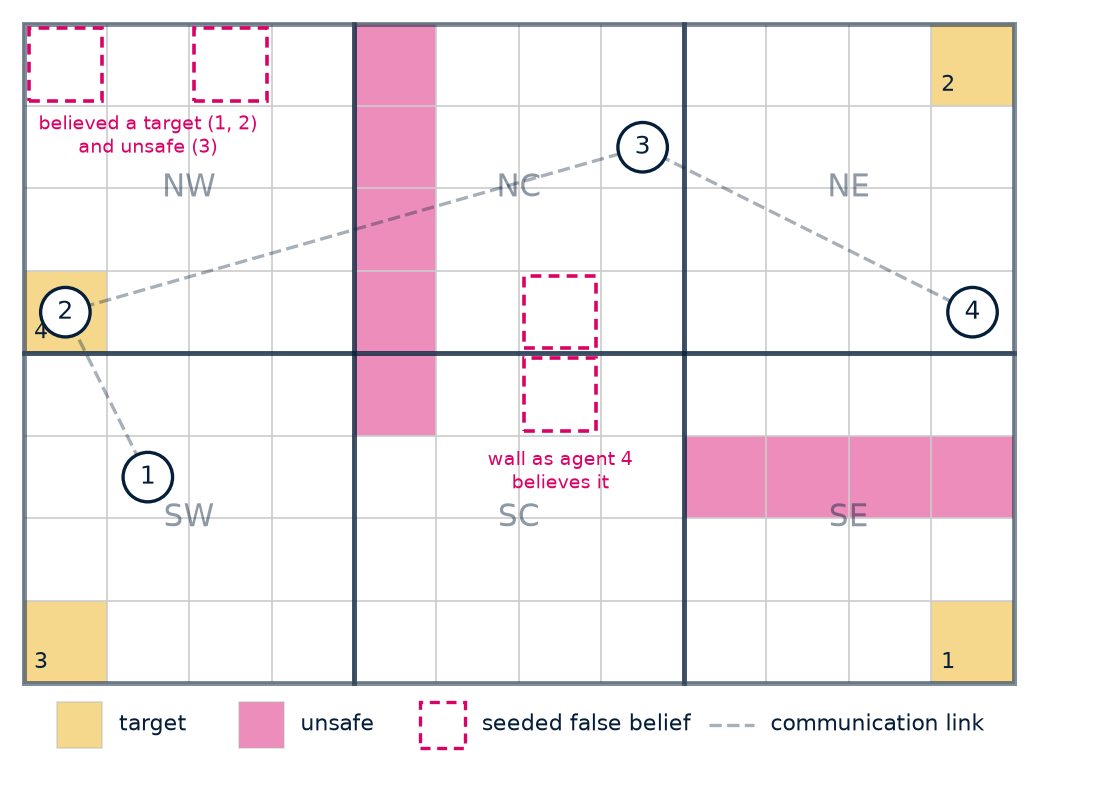
\includegraphics[width=0.56\textwidth]{world.pdf}
\caption{The demonstration world: a $12 \times 8$ grid ($\approx$0.2\,m tiles on the 3.2\,m$\,\times\,$2.0\,m arena), six region-rooms. Solid fills are ground truth (gold targets, pink hazard walls); dashed outlines are seeded \emph{false} beliefs, annotated by holder; gray dashes are the communication chain.}
\label{fig:world}
\end{figure}

The scenario instantiates the search-and-neutralize vignette of the proposal at arena scale. Four UGVs are assigned distinct target squares in the four quadrants of \Cref{fig:world}; the ground truth holds two hazard walls; each agent is seeded a mixture of correct and incorrect beliefs about hazards, targets, and \emph{where its teammates were sent}: precisely the disagreements about information and goals the flow must resolve. Three seeded conflicts drive the drama.
\begin{description}[itemsep=1pt, topsep=3pt]
\item[Region-level conflict.] Agents 1 and 2 believe targets stand in the northwest room where Agent 3 believes hazards: a genuine region-level conflict the interfaces must reconcile.
\item[Diameter-length correction.] Agent 4 has the central hazard wall in the wrong column, two tiles east of the truth, so left alone it detours around empty ground and drives into the real wall. Only Agent 1 knows better, three hops away, so the correction must traverse the network's diameter.
\item[Disagreement below the vocabulary.] The partition places both walls \emph{interior} to their rooms: the true wall and Agent 4's misplaced one flag the \emph{same} regions, so at the interface's resolution Agent 4 is not even wrong. The sections close over the tile-level disagreement, the abstraction earning its keep on camera.
\end{description}
Communication is intermittent by construction (sweeps on a coarse clock and on planning events; asynchronous departures under a round-robin schedule), exercising the schedule-independence guarantee of \Cref{sec:sheaves} under partial firing sets. The design comprises three arms, identical in all but one respect (\Cref{tab:arms}); scoring awards $+5$ per target reached, $+1$ per safe tile, $-2$ per truly-unsafe tile entered.

\begin{table}[h]
\centering
\small
\begin{tabular}{lll}
\toprule
\textbf{Arm} & \textbf{Configuration} & \textbf{What it isolates}\\
\midrule
Contract sheaf (demo) & six-region mission sheaf, monitor on & abstraction + contracts + flow\\
No abstraction & identity partition ($\rho = \mathrm{id}$, bijective restrictions) & value of the region vocabulary\\
No communication & communication disabled & value of communicating at all\\
\bottomrule
\end{tabular}
\caption{The three arms, which differ in exactly one configuration each. World, starts, assignments, beliefs, topology, planner, and scoring are held fixed.}
\label{tab:arms}
\end{table}

\subsection{Execution of the Robot Experiments (Subtask 5.2)}
\label{sec:task52}

\prompt{Run the experiments on UGVs, collecting data and videos showing task resolution despite degraded conditions.}

All three arms have been executed end-to-end: first in the Robotarium simulator via the exact submission bundles of \Cref{sec:task43}, and subsequently on the physical testbed, whose returned overhead footage (August 12, 2026) is the record of this subtask. Wall-clock durations sit comfortably under the portal's 600\,s cap: 133\,s (demonstration), 123\,s (no abstraction), and 76\,s (no communication). \Cref{fig:stills} shows four moments of the demonstration arm as filmed from overhead, the experiment's figure projected on the arena floor beneath the robots; \Cref{tab:runstats} summarizes the run twice over, by the self-describing JSON log of the simulator execution and by the testbed's returned console log, which records the same event stream (sweep captions, assumption violations, recommitments) the simulator log does. The two executions tell the same story with the small divergences physical timing buys: the first global section closes with \emph{exactly} 39 tiles in dispute in both, the section indicator cycles eight times in both, and the testbed run settles at 73 sweeps on 95 differing tiles against the simulator's 77 and 96; the physical run's higher violation and recommitment counts (52 and 27, against 38 and 19) are the negotiation replaying under asynchronous arrival order. One honest caveat: the testbed's JSON itself was not written, because a final diagnostic print crashed on a simulator-only attribute after the experiment completed but before the log closed; the print is now guarded and moved after the close, so a resubmission would return the JSON for the exact tile-for-tile check.

\begin{figure}[t]
\centering
\begin{tabular}{cc}
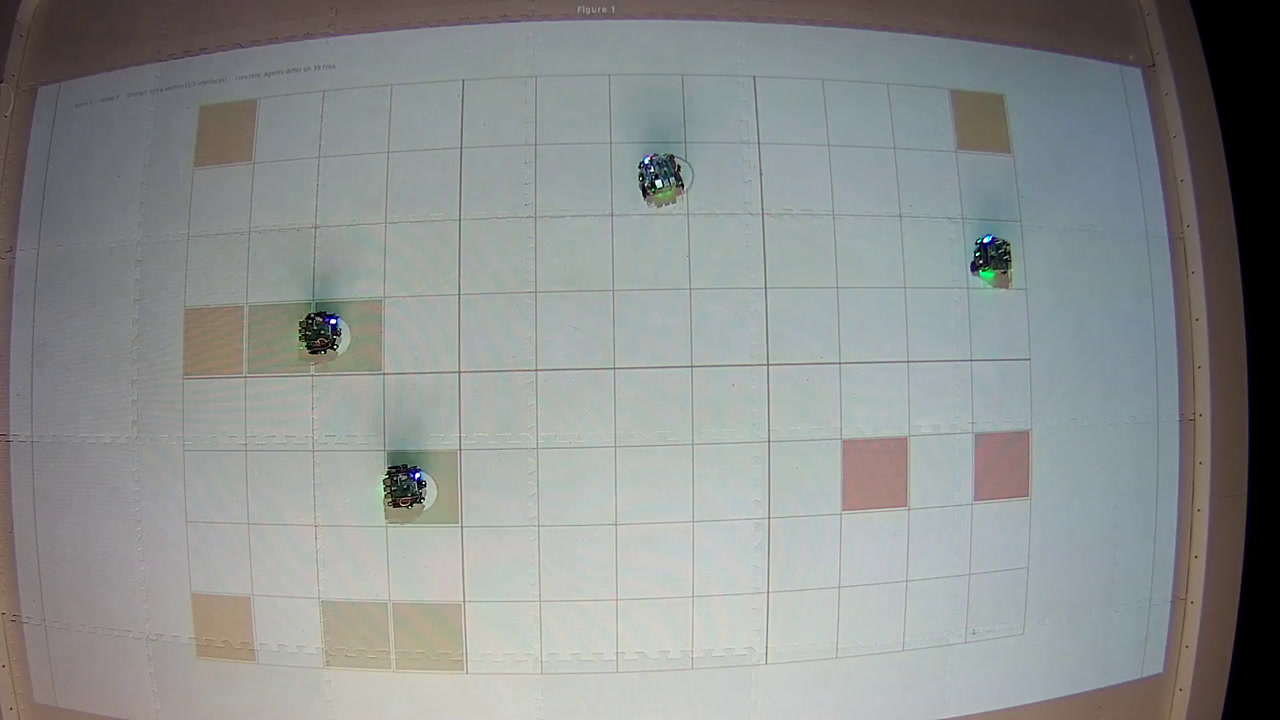
\includegraphics[width=0.42\textwidth]{phys_still_opening.jpg} &
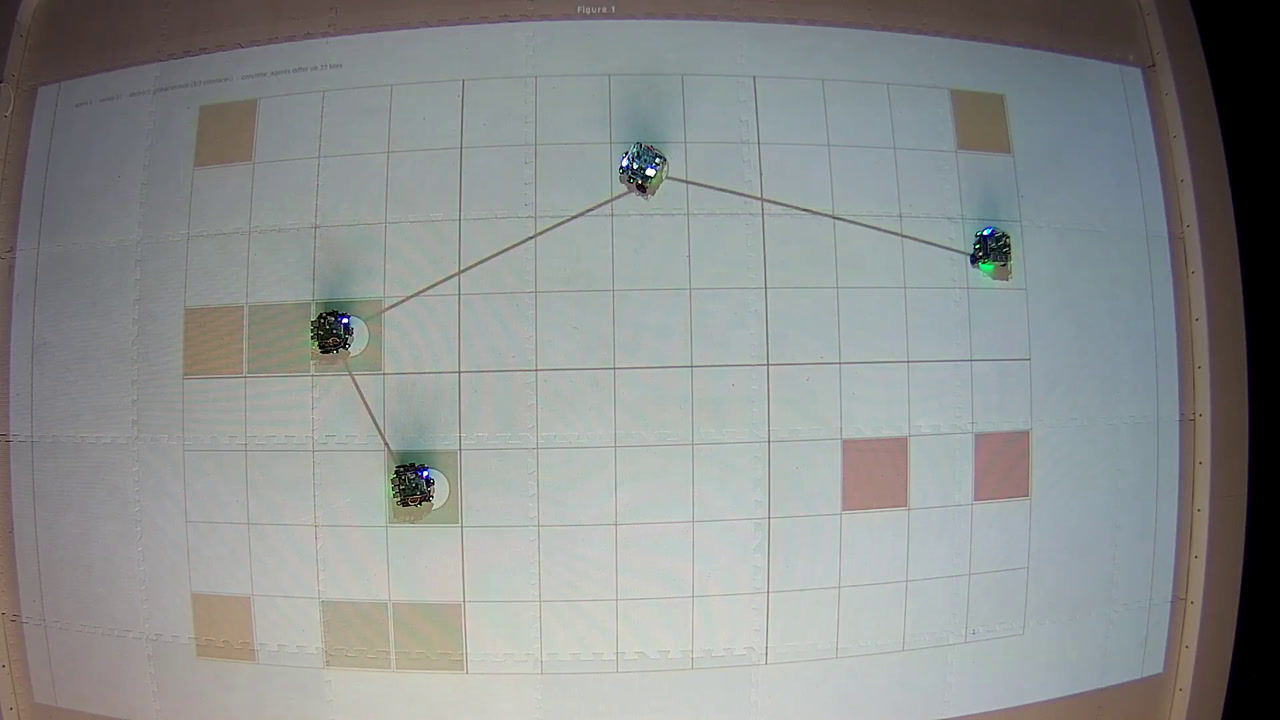
\includegraphics[width=0.42\textwidth]{phys_still_first_section.jpg}\\
{\footnotesize (a) $t \approx 50$\,s: flow in progress} & {\footnotesize (b) $t \approx 54$\,s: first global section}\\[3pt]
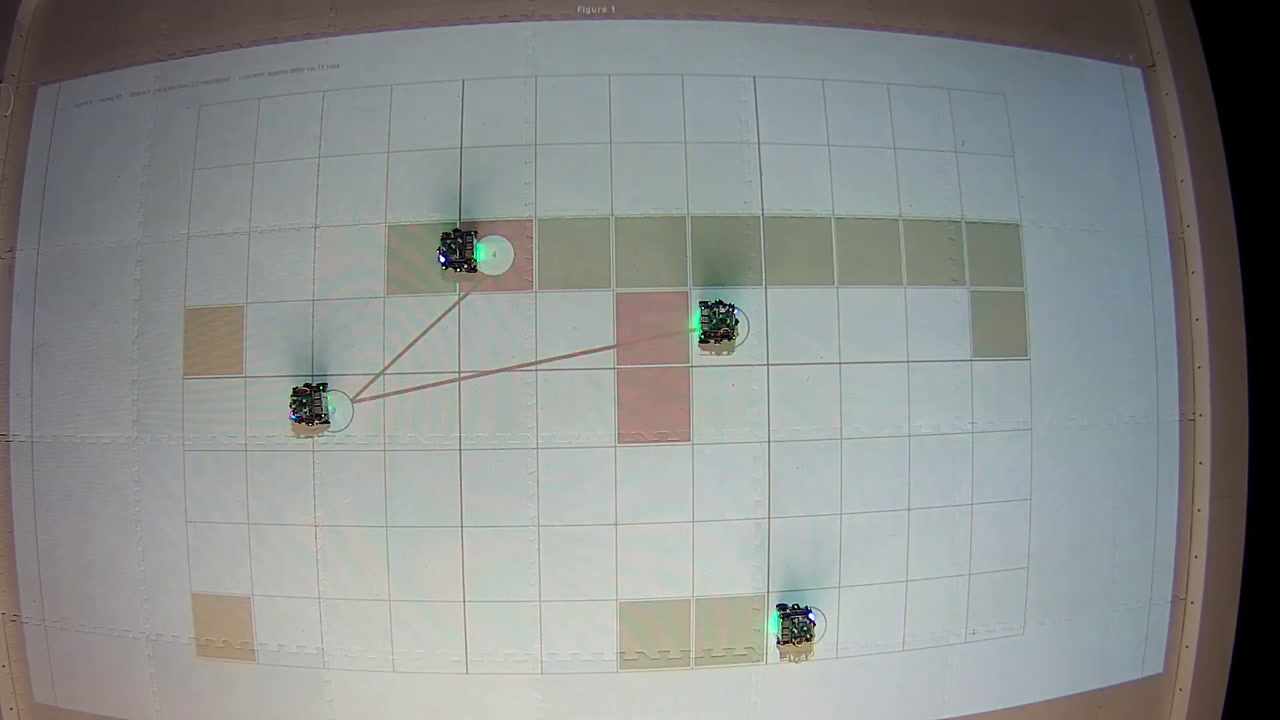
\includegraphics[width=0.42\textwidth]{phys_still_reopened.jpg} &
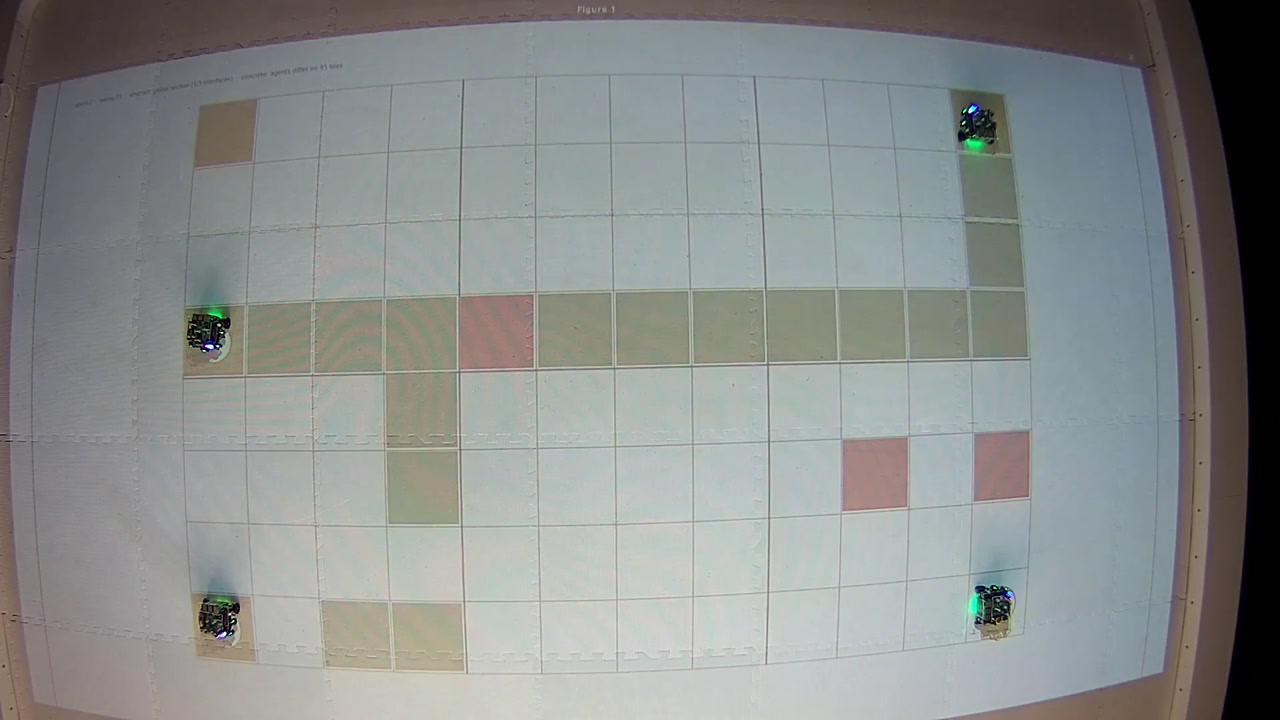
\includegraphics[width=0.42\textwidth]{phys_still_settled.jpg}\\
{\footnotesize (c) $t \approx 100$\,s: reopened by recommitment} & {\footnotesize (d) $t \approx 125$\,s: settled, all agents home}\\
\end{tabular}
\caption{Overhead-camera stills of the demonstration arm executed on the physical Robotarium testbed (returned footage of August 12, 2026). The projected figure beneath the robots shows the toured agent's beliefs as tile fills, links drawn between robots where the interface agrees, and the two-level caption line (\emph{abstract: global section? / concrete: tiles differing}). (b) is the first global section (sweep 10 by the returned console log, \emph{with the agents still differing on 39 tiles}); (d) is the settled end state, a global section over 95 tiles of residual concrete disagreement, every robot on its assigned square.}
\label{fig:stills}
\end{figure}

The demonstration run resolves every seeded disagreement and delivers all four agents home. Three behaviors deserve narration.
\begin{description}[itemsep=1pt, topsep=3pt]
\item[Abstract agreement over concrete disagreement.] The first global section arrives at sweep 8 with 39 tiles still disputed, and the run \emph{ends} on a section with 96: the partition, not attrition of differences, is what agreement means here.
\item[Contract-driven rerouting.] The monitor read out 38 assumption violations, agents recommitted 19 times, and each recommitment lawfully reopened closed sections that the flow then re-closed; the section indicator cycled eight times, the negotiation made visible.
\item[Observation as arbiter.] 51 of 208 arrival observations carried news, including those that corrected Agent 4's misplaced wall as the network's truth reached it hop by hop. At the very end the arriving agents retract their claims, briefly reopening the flow; the closing hold gives the final sweeps their seconds on the floor, and the run closes on the re-established section of \Cref{fig:stills}(d).
\end{description}

\begin{table}[h]
\centering
\small
\begin{tabular}{lrr}
\toprule
\textbf{Quantity} & \textbf{Simulator} & \textbf{Testbed}\\
\midrule
agents / arrived & 4 / 4 & 4 / 4\\
movement events & 52 & ---\\
mission score (per agent) & 59 (16/15/14/14) & ---\\
assumption violations read & 38 & 52\\
arrival observations (carrying news) & 208 (51) & ---\\
Laplacian sweeps & 77 & 73\\
first global section & sweep 8 & sweep 10\\
tiles disputed at first section & 39 & 39\\
section closed/reopened & 8 times & 8 times\\
recommitments & 19 & 27\\
tiles disputed at end & 96 & 95\\
wall-clock duration & --- & 133\,s\\
\bottomrule
\end{tabular}
\caption{The demonstration arm twice over (submitted bundle, seed 0): the simulator execution by its JSON log, the physical execution by its returned console log and footage. Dashes are quantities the console log does not speak to; the testbed JSON was lost to the diagnostic-print crash described in the text.}
\label{tab:runstats}
\end{table}

\task{Remaining physical artifacts (TBD): (i) portal confirmation numbers for the three submissions; (ii) optionally, one resubmission of the demonstration arm with the repaired logging, to retrieve the JSON for the exact tile-for-tile parity check the console-log comparison of \Cref{tab:runstats} approximates. Durations, overhead stills, projection legibility, and the event-stream comparison are in hand from the returned footage and console logs of August 12, 2026.}
\ai{I extracted the four stills of \Cref{fig:stills} from \texttt{exp/robotarium/\_videos/Contract sheaf~-~4 robots, 12x8, 6 regions~-~08-12 01:48.mp4} at $t \approx 50, 54, 100, 125$\,s, choosing the moments by reading the projected caption line frame by frame; durations come from the video lengths, and the testbed column of \Cref{tab:runstats} from the console logs you dropped in \texttt{exp/robotarium/logs/}. All three logs end in the same crash: \texttt{main.py} line 728's \texttt{DURATION\_SECONDS} print reads \texttt{robotarium.\_iteration}, which only the local simulator fork has, and it fired \emph{before} \texttt{experiment\_log.close()}, which is why no JSON came back. I fixed \texttt{experiment\_template.py}: the log now closes first and the print is guarded. Rebuilding the bundles picks the fix up.}

\subsection{Benchmark Against MARL (Subtask 5.3)}
\label{sec:task53}

\prompt{Implement a MARL baseline and compare its performance (e.g., time to completion, efficiency) with SEAMAN under identical conditions.}

The benchmarking protocol is \emph{paired}: every policy runs the same sampled world with identical starts, beliefs, assignments, and topology, so any difference in outcome is attributable to the single policy ingredient that changed. A headless harness executes the protocol at scale, at present comparing three policies: \textsf{isolated} (no communication), \textsf{sheaf} (one Laplacian sweep per step), and \textsf{omniscient} (ground truth handed to every agent: the ceiling communication is trying to reach, not a runnable policy, included so a score difference reads as a fraction of what was there to be had). \Cref{tab:benchmark} reports the sweep over initial knowledge density: communication recovers 26\%, 50\%, and 75\% of the isolated-to-omniscient score gap as agents start knowing 10\%, 20\%, and 40\% of the world. The recovery is monotone in knowledge, as the flow can only redistribute what somebody knows. Full grids and the arrival-rate discussion are in \Cref{sec:app-benchmark}.

\begin{table}[h]
\centering
\small
\begin{tabular}{lccc@{\qquad}ccc}
\toprule
& \multicolumn{3}{c}{\textbf{mission score}} & \multicolumn{3}{c}{\textbf{final belief coverage}}\\
\textbf{knowledge} & \textsf{isolated} & \textsf{sheaf} & \textsf{omniscient} & \textsf{isolated} & \textsf{sheaf} & \textsf{omniscient}\\
\midrule
10\% & 12.4 & 21.7 & 48.1 & 0.10 & 0.40 & 1.00\\
20\% & \phantom{0}7.2 & 29.0 & 51.2 & 0.20 & 0.64 & 1.00\\
40\% & 25.9 & 44.3 & 50.5 & 0.41 & 0.89 & 1.00\\
\bottomrule
\end{tabular}
\caption{Paired benchmark, 40 worlds per row (4 agents, $9 \times 5$ grids, error-free beliefs): mean score and coverage.}
\label{tab:benchmark}
\end{table}

The MARL baseline slots into this harness as a fourth policy: a centralized-training, decentralized-execution policy (independent PPO with parameter sharing as the reference configuration) trained on the mission score as its reward, observing exactly what a SEAMAN agent observes (own beliefs, own position, messages from graph neighbors only), and evaluated on held-out worlds under the identical paired protocol. Its implementation is in progress and its numbers wait in the wings; we note the structural contrast the comparison is designed to expose: MARL amortizes coordination into weights offline and offers no per-run certificate, whereas SEAMAN's is computed online with a checkable one: the run \emph{knows} when its interfaces agree, and \Cref{tab:runstats} is that knowledge in a table.

\task{MARL numbers (TBD): algorithm and training budget as run, seeds, and the paired table extending \Cref{tab:benchmark} --- time to completion, score, unsafe entries, arrival rate --- under identical worlds and communication constraints.}

%%%%%%%%%%%%%%%%%%%%%%%%%%%%%%%%%%%%%%%%%%%%%%%%%%%%%%%%%%%%%%%%%%%%%%%%%%%%%%%%%%%
\nocite{*}
\bibliographystyle{plainnat}
\setlength{\bibsep}{2.5pt}
{\footnotesize
\bibliography{report}
}
%%%%%%%%%%%%%%%%%%%%%%%%%%%%%%%%%%%%%%%%%%%%%%%%%%%%%%%%%%%%%%%%%%%%%%%%%%%%%%%%%%%

%%%%%%%%%%%%%%%%%%%%%%%%%%%%%%%%%%%%%%%%%%%%%%%%%%%%%%%%%%%%%%%%%%%%%%%%%%%%%%%%%%%%%%%
\appendix
\section{Additional Experimental Details}
\label{sec:appendix}

\subsection{Emperical Convergence Analysis}
\label{sec:app-convergence}

Disagreement is measured throughout this appendix as follows. Writing $C = (A_C, G_C)$, a contract denotes the pair of state sets $(\llbracket A_C \rrbracket, \llbracket \sat{G}_C \rrbracket)$, and the \emph{symmetric distance} between $C, D \in \Con{\Sigma}$ is
\begin{equation*}
d(C, D) \;=\; \tfrac{1}{2}\Bigl(\mu\bigl(\llbracket A_C \rrbracket \,\triangle\, \llbracket A_D \rrbracket\bigr) + \mu\bigl(\llbracket \sat{G}_C \rrbracket \,\triangle\, \llbracket \sat{G}_D \rrbracket\bigr)\Bigr) \;\in\; [0, 1],
\end{equation*}
where $\mu$ is the uniform probability measure on the states of $\Sigma$ and $\triangle$ the symmetric difference; $d(C, D) = 0$ exactly when $C = D$ as saturation classes. The \emph{Tarski--Dirichlet energy} of an assignment $x$ is its total disagreement across interfaces, measured where the sheaf condition \eqref{eq:section} lives,
\begin{equation}
\label{eq:energy}
\mathcal{E}(x) \;=\; \sum_{ij \in E} d\bigl((R_{i \face ij})_{!}\, x_i,\; (R_{j \face ij})_{!}\, x_j\bigr),
\end{equation}
so that $\mathcal{E}(x) = 0$ exactly on global sections: the order-theoretic counterpart of the quadratic form $x^{\top}\!\Lap x$ whose decay tracks classical heat flow. Over the mission sheaf the interface alphabet is a product over regions, and the sum in \eqref{eq:energy} refines to (interface, region) components.

A randomized-ensemble campaign ran all four flows (primal and dual, along each adjunction of \eqref{eq:adjunctions}) under four firing schedules across five studies (topology, scale, coarseness, encoding, canonicalization): 564 runs, of which all 561 within the solver budget converged (mean 3.3 sweeps, maximum 21), every monotonicity and section invariant intact, the greatest distance between two schedules' limits exactly zero across all 24 (sheaf, flow) groups, and concrete disagreement at the limit growing with the coarseness of the summary while abstract disagreement stayed identically zero.

Rather than plot that ensemble's statistics, \Cref{fig:energy} hones in on one \emph{replayable} instance of the demonstration construction itself, scaled from four agents to a network of 32 (\texttt{exp/scale\_example.py}, seed 0): the six-room $12 \times 8$ world of \Cref{sec:task51}; beliefs sampled at 20\% knowledge with 10\% error by the \Cref{sec:task53} sampler; mission contracts \eqref{eq:mission} with reliance and exclusive claims from planned corridors; and the closed-form $R_{!}$ transports of \Cref{sec:task42} along the region-summary restrictions \eqref{eq:summary}, over a random spanning tree with two chords: 33 interfaces, diameter 14, $33 \times 6 = 198$ interface--region components. The synchronous flow closes 157 of the 198 components on its first sweep and reaches a global section at sweep 6, well inside the diameter bound, the Tarski--Dirichlet energy \eqref{eq:energy} falling monotonically through three decades, from 10.1 to exactly zero at that sweep; the fixed point is certified two sweeps later, at a mean of 2.2\,s per sweep (maximum 6.6\,s, the first) for the whole 32-agent network. The right panel is the abstraction claim at scale: the section closes over 1{,}084 tile-level differences between neighboring agents' beliefs, and not one of them moves. What the agents still disagree about lives entirely in the kernel of the summary, which is precisely what the region vocabulary was chosen to tolerate.

\begin{figure}[t]
\centering
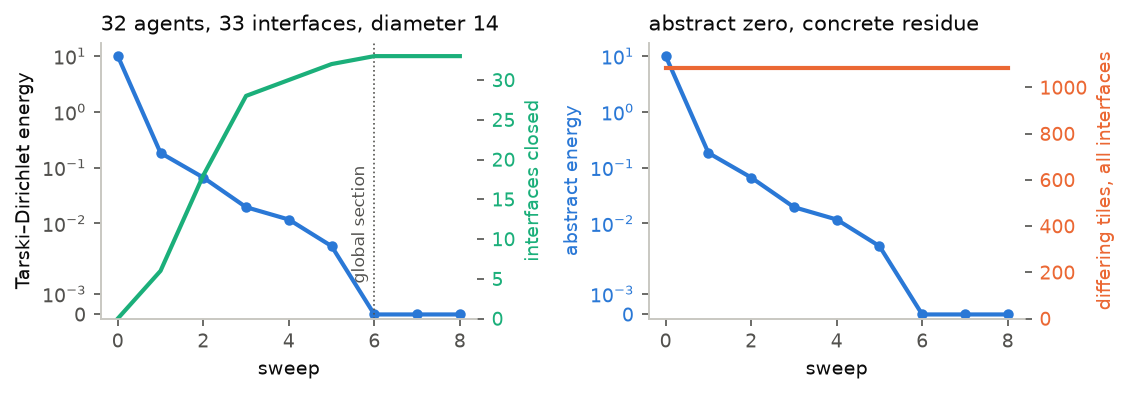
\includegraphics[width=0.94\textwidth]{scale_energy.pdf}
\caption{One randomized, replayable instance of the demonstration construction at network scale (32 agents, seed 0; \texttt{exp/scale\_example.py}). Left: Tarski--Dirichlet energy of the synchronous primal flow per sweep, with the count of closed interfaces; the dotted line marks the first global section (sweep 6, against a diameter bound of 14). Right: the same energy against the number of tiles on which neighboring agents' beliefs differ, which the flow never moves: abstract agreement is reached \emph{over}, not by eliminating, concrete disagreement.}
\label{fig:energy}
\end{figure}

\subsection{Validation on the Demonstration Sheaf}
\label{sec:app-validation}

Independently of the ensemble, the flow was validated on the demonstration's own sheaf construction from 15 sampled initial assignments on each of four topologies (path, cycle, star, complete), each run under synchronous, round-robin, and random schedules. Monotonicity, the independently-computed closed-form limit (pointwise intersection of initial possibility masks over each connected component), and no-collapse held in 60 of 60 trials; the limit was verified a global section, identical across schedules, in 57 of 60 (path 13/15, cycle 14/15, star and complete 15/15), the residual three under investigation. The synchronous flow reached its fixed point within the graph diameter on every trial: the bound that sizes how long a demonstration must let the robots listen.

\subsection{Additional Benchmark Details}
\label{sec:app-benchmark}

The harness behind \Cref{tab:benchmark} also swept belief error rates (0--30\%) at each knowledge level: the sheaf's score advantage over \textsf{isolated} persists at every cell, narrowing as error rises, since the flow faithfully propagates wrong pins along with right ones. One honest caveat: arrival \emph{rate} dips slightly under \textsf{sheaf} (0.74 vs.\ 0.93 at knowledge 20\%), as does, tellingly, \textsf{omniscient} (0.78), because better-informed agents detour along the same safe corridors and meet there: a standoff of shared knowledge, not of the flow, and precisely what the exclusive-claims machinery of \Cref{sec:task41} breaks; the demonstration arm deadlocks nowhere.

\label{sec:app-behaviors}Three behaviors of the demonstration arm merit record. (i) \emph{Early route flapping:} before the network's knowledge hardened, one agent alternated between two near-equal-cost corridors (11 of the 19 recommitments): the finite penalty behaving as designed, but pricing a recommitment hysteresis as worthwhile tuning. (ii) \emph{End-of-run reopening:} arriving agents retract their claims, so the final arrivals lawfully un-close sections the flow re-closes on the fully-arrived state. (iii) \emph{Region-level absorption:} no fused summary ever entailed a label both flagged and excluded, and no stalk collapsed to a lattice extreme: disagreement lived its whole life inside the lattice, the design's central claim about itself.

%%%%%%%%%%%%%%%%%%%%%%%%%%%%%%%%%%%%%%%%%%%%%%%%%%%%%%%%%%%%%%%%%%%%%%%%%%%%%%%%%%%


\end{document}
